\section{Proactive Approaches}
Proactive approaches aim at lowering the possibility of Tor users being affected by an active BGP routing attack on Tor relays. Network-level adversaries can announce a more-specific prefix to hijack the traffic between the client and the Tor guard relay; further more, the adversaries can also announce an equally-specific prefix to achieve the same goal for a portion of Tor clients on the internet. To counter these two attack strategies, we propose two methods, respectively: 1) convincing relay operators to announce the relay in a /24 prefix to defend against a more-specific prefix attack, 2) introducing a new Tor guard relay selection algorithm that minimizes the likelihood that a Tor client sees a hijacked route in the case that her guard is hijacked by an equally-specific prefix attack.

\subsection{Using /24 Prefixes}
\label{subsec:24prefix}

Sun \emph{et al.} \cite{sun2015raptor} recently found that more than 90\% of BGP prefixes hosting relays are
shorter than /24, making them vulnerable to a more-specific BGP prefix attack. Thus, one quick way to make Tor relays more resilient to such active routing attacks is to announce /24 prefix covering Tor relays. In order to make real world impact of this approach, we start a campaign by contacting network operators whose prefixes contain Tor relays, and asking them to announce a more specific /24 prefix covering the relay. 

We start by cooperating with Princeton University, which contains a Tor relay under a /16 prefix. 

\subsection{Guard Relay Selection}

Guard relay is at an important position that it has direct connection with the Tor client. It has been shown that network-level adversaries can launch a more-specific BGP prefix attack to hijack the Tor traffic from the guard relay to the malicious AS \cite{sun2015raptor}, and this can be potentially prevented by advertising /24 prefixes, as discussed in Section ~\ref{subsec:24prefix}. However, even if the guard relay belongs to a /24 prefix, it is still subject to an equally-specific prefix attack. Unlike more-specific attacks which spread through the whole internet, equally-specific attacks can only affect connections within a small range - i.e., ASes that have more preferred paths to the hijacking AS than the true origin AS. Thus, picking a Tor guard relay that has relatively high AS resiliency against such equally-specific attacks could protect Tor clients from being affected and deanonymized by network-level adversaries. Therefore, we propose a new guard relay selection algorithm that incorporates this aspect.

\subsubsection{Design Goals}
\begin{enumerate}
\item \emph{Deal with the possibility of prefix hijacks.} This is the main goal of the new guard relay selection algorithm. The algorithm computes the AS resiliency against prefix hijacks of all Tor guard relays from the client source AS, and prefers the ones that have higher resiliencies, minimizing the likelihood that the client would be affected by a prefix hijack on her guard relay. 
\item \emph{Protect the anonymity and privacy of Tor clients.} The algorithm should provide a good variance in its probabilities of selecting relays, i.e., avoid favoring certain relays much more than all other ones. Also, the algorithm should not expose the Tor clients to new attacks, such as fingerprinting attacks which might deanonymize the clients by observing their relay selection preferences. 
\item \emph{Load balance Tor traffic.} The algorithm should incorporate relay bandwidth into selection decision and avoid causing excessive traffic congestion on low bandwidth relays. 
\item \emph{Performance overhead.} The algorithm should have a reasonable computation overhead over the vanilla Tor algorithm when bootstrapping, and fast page load time using its constructed circuit of relays. 
\end{enumerate}

\subsubsection{Minimize the possibility of being affected by prefix hijacks}

Recall from Section ~\ref{hijack_methodology} that we sum up the resiliency from \emph{each} source AS to obtain the total resiliency for the Tor-related ASes. However, from the perspective of a Tor client, the client would only care about the resiliency of a Tor-related AS from where the client is located as the source AS instead of the total resiliency. Thus, we use Algorithm ~\ref{algo:calcres} to calculate resiliency $R(i)$ of each Tor-related AS $i$, from the client AS $t$. 

Tor relay selection has been bandwidth-aware and prefers high bandwidth relays. The probability of each relay $i$ being chosen is based on its bandwidth $B(i)$. Thus, in order to still provide clients with the load balancing option of Tor bandwidths, we offer a tunable parameter $\alpha$ in the relay selection algorithm combining AS resiliency $R(i)$ and bandwidth $B(i)$. Each relay $i$ will be assigned a weight as following:
\begin{equation*}
W(i) = \alpha \times R(i) + (1 - \alpha) \times B(i)
\end{equation*}
Note that, when $\alpha$ is set to $0$, the relay selection becomes the same as bandwidth-only selection; while when $\alpha$ is set to $1$, the selection becomes resiliency-only selection. 

\subsubsection{Protect the anonymity of clients}

If we simply select the set of guard relays based on the probability of $relay\_weight/total\_weight$, an adversary can potentially run a relay that is close enough to the Tor client, such that it has high resiliency from the client AS as the source, and thus obtains high probability of being chosen. Further more, the Tor client could also be susceptible to fingerprinting attacks due to the differences in relay selection probabilities based on AS-location of the client. An adversaries that can observe the client for a long enough time may be able to infer the AS-location of the client based on its observed relay selection choices. Thus, we need to take into account these potential vulnerabilities and protect the anonymity of clients. 

Instead of selecting relay directly based on its weight, we will first select a cluster of 
\begin{equation*}
m + \alpha \cdot g \cdot (N - m)
\end{equation*}
number of relays, in which $m$ is the minimum number of relays needed (i.e., 1 for single guard and 3 for multiple guards), $N$ is the total number of relays and $g$ is a configurable parameter indicating the maximum percentage of additional relays we want to pick into the cluster. Then, we will pick the guard relay(s) at random from the cluster. Note that when $g$ is set to $0$, then no additional randomization will be performed, while if $g$ is set to $1$, all guard relays will be picked randomly regardless of bandwidth or resiliency. We will evaluate how different values of $g$ may impact the security and anonymity.

\subsubsection{Implementation on Tor}
Mapping the IP addresses of the Tor client and Tor relays to ASN would be necessary before we can compute AS resiliency. In order to preserve the anonymity of the Tor client and not reveal its location to outside servers or anyone who can observe the its communications, the client will perform the IP to ASN mapping locally by utilizing the Maxmind ASN database (citation here). Note that the vanilla Tor client also uses the Maxmind GeoIP database for IP to Country mapping. In addition, the client will use the AS topology database from CAIDA (citation here) for AS-level path inference in the resiliency calculation. 

If the Tor client specifies in the torrc configuration file that the AS resiliency-aware guard relay selection is preferred, and supplies an $\alpha$ value as the tunable parameter, the following procedure will be invoked:

\begin{enumerate}
\item If the Maxmind ASN file and AS topology file have not been cached, the Tor client will download the two file from Maxmind and CAIDA, respectively, and save them in the local data directory. 
\item The Tor client will perform IP to ASN mapping, and compute the AS resiliency of all candidate relays from the client AS as the source AS. 
\item The Tor client will compute a weight for each candidate relay using formula $W(i) = \alpha \times R(i) + (1 - \alpha) \times B(i)$. 
\item The Tor client will select a cluster of $m + \alpha \cdot g \cdot (N - m)$ relays based on their weights, and then randomly select the guard relay(s) from the cluster. 
\item The Tor client will proceed with the path selection. The remaining part of the circuit construction process stays the same as it is in Tor. 
\end{enumerate}

\subsection{Relay Selection Evaluation}

We evaluate the AS resilience based relay selection from performance and security perspectives. 

\subsubsection{Performance Evaluation}

First, we evaluate the runtime of the AS resilience calculation given a source AS. We pick $1000$ ASes randomly as the source AS, and record how much time it takes each of them to complete the calculation. Figure ~\ref{fig_ascal} show the CDF of the runtime of AS resilience calculation. Most of the source ASes finish within $0.6$ second. 

\begin{figure}[ht!]
\centering
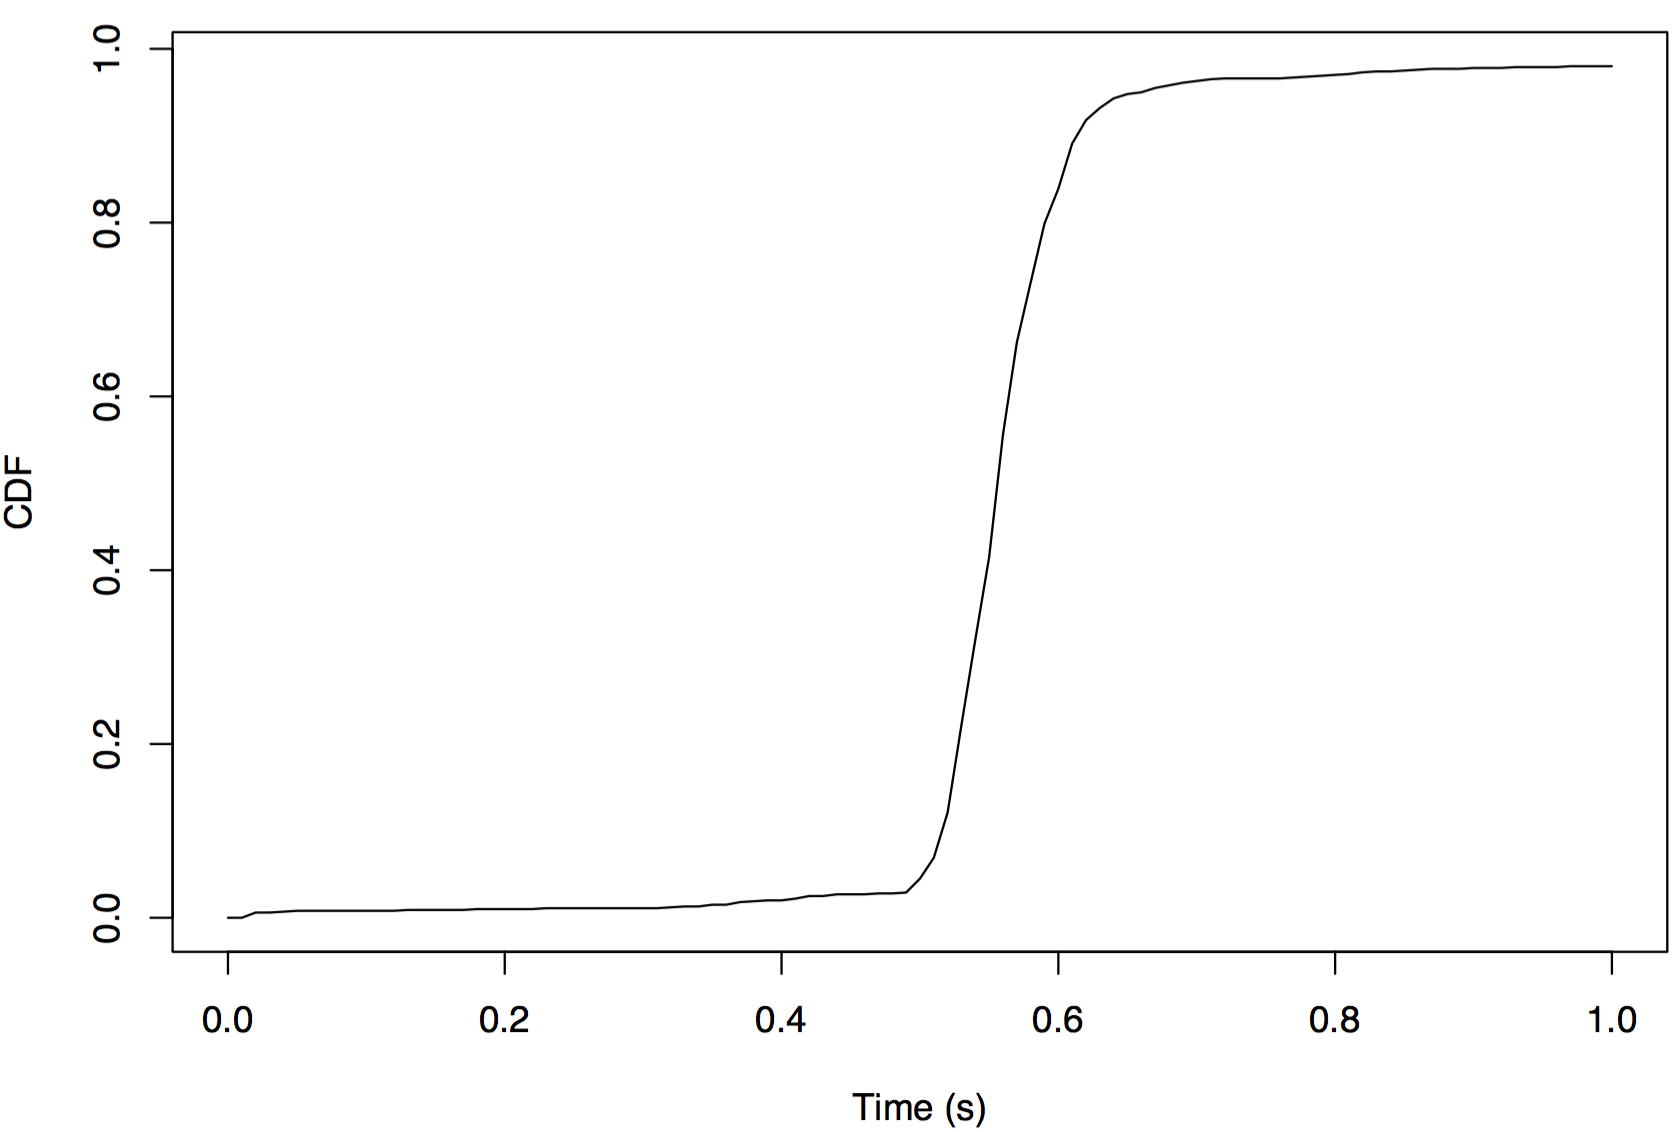
\includegraphics[width=80mm]{figure/runtime}
\caption{Runtime of AS resilience calculation from a given source AS \label{fig_ascal}}
\end{figure}

[NOTE: more evaluation here on Shadow and real world run]

\subsubsection{Security Evaluation}

\textbf{Relay selection variance} in entropy can be evaluated using Gini coefficient as the entropy evaluation metric, as it has been used in previous work to measure anonymity selection in Tor ~\cite{akhoondi2012lastor}. We first evaluate it without doing the clustering, for five values of $\alpha: \{0, 0.25, 0.5, 0.75, 1\}$ with $1000$ randomly selected ASes as source AS. Note that when $\alpha = 0$, it is equivalent to bandwidth-based selection. Figure ~\ref{fig_gini} shows the result. The green line to the right is when $\alpha = 0$, so it's solely based on bandwidth resulting in a Gini coefficient of $0.607$ for all source ASes. 

\begin{figure}[ht!]
\centering
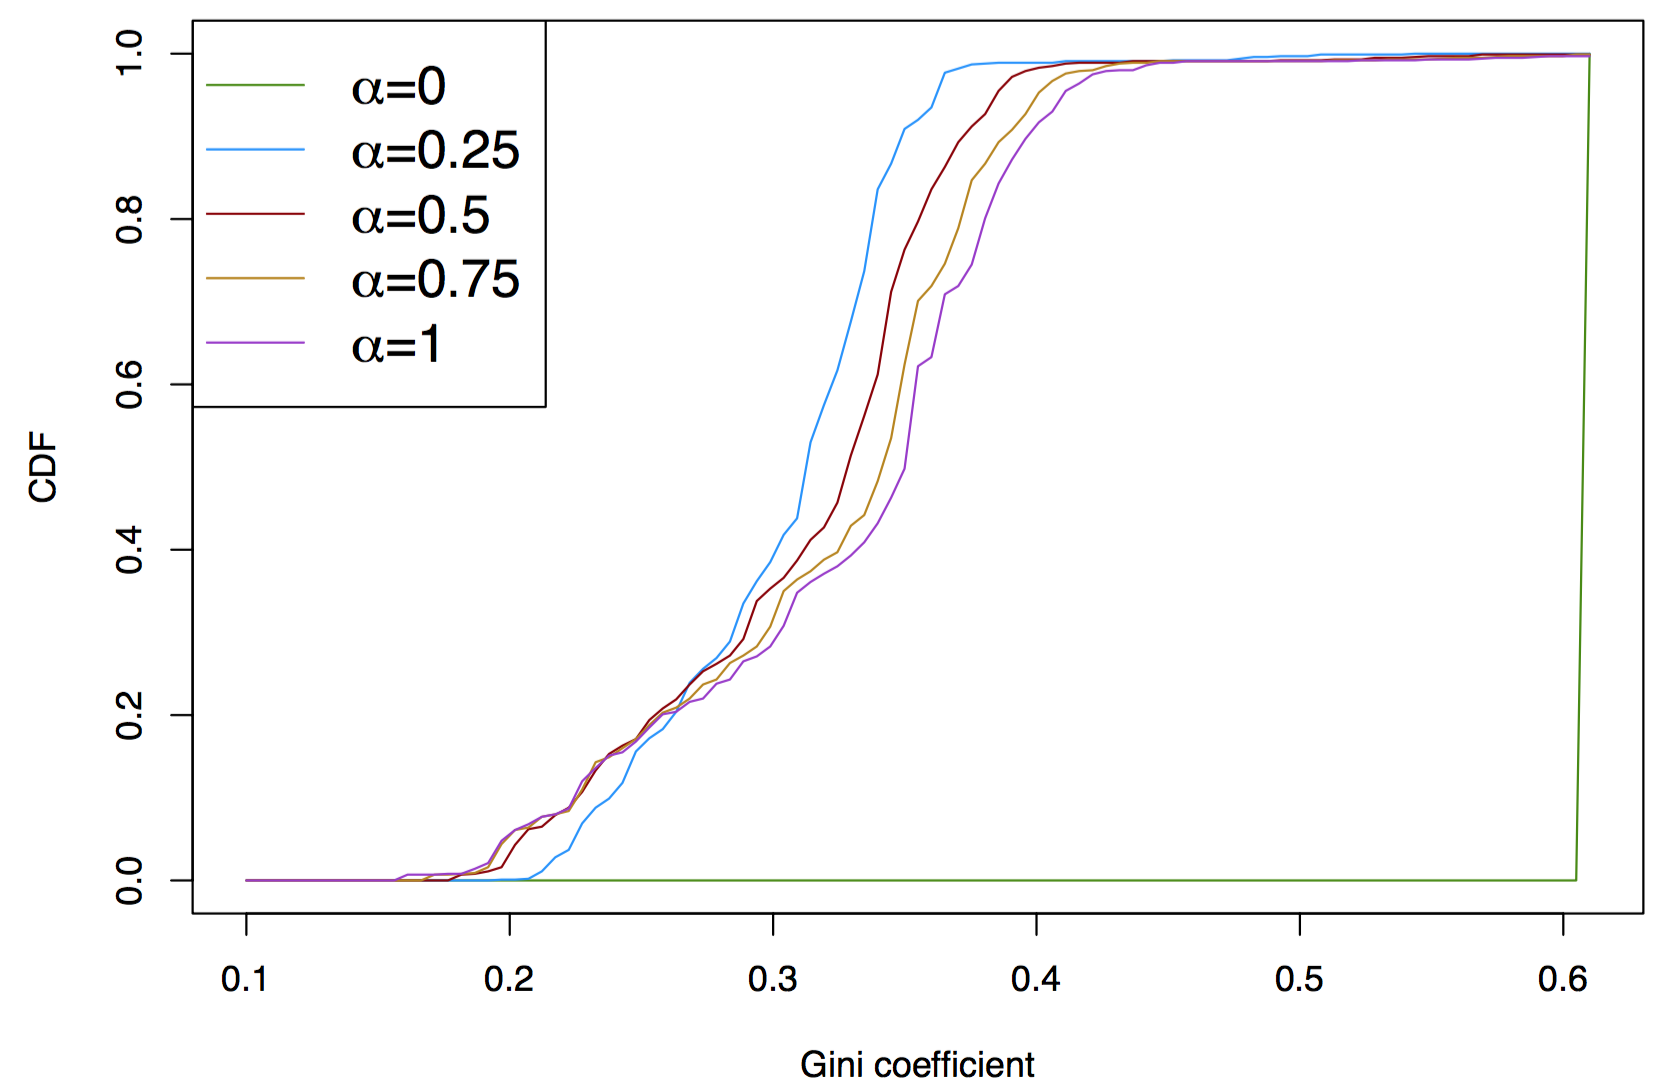
\includegraphics[width=80mm]{figure/gini}
\caption{Gini coefficients with different $\alpha$ values \label{fig_gini}}
\end{figure}

The Gini coefficients for the other four $\alpha$ values which involve resilience-based selection are much lower than bandwidth-based selection, meaning that there is higher entropy and lower skew in probabilities of selecting any particular relay. However, the variance in relay selection probability \emph{across} different source ASes is bigger than bandwidth-only: when $\alpha = 0$, all sources ASes have the same gini coefficient of $0.607$, while for other $\alpha$ values, the gini coefficient could vary from approximately $0.2$ to $0.4$, depending on the source AS. 

[NOTE: more evaluation on effect of g here]\\

\textbf{Probability of being affected by a hijack attack} is evaluated by the sum of \emph{Probability(choose relay $i$) * Probability(client is affected if relay $i$ is hijacked)} for all candidate relay $i$. Again, we first evaluate it without doing the clustering, for five values of $\alpha: \{0, 0.25, 0.5, 0.75, 1\}$ with $1000$ randomly selected ASes as source AS. Figure ~\ref{fig_attack} shows the result. 

\begin{figure}[ht!]
\centering
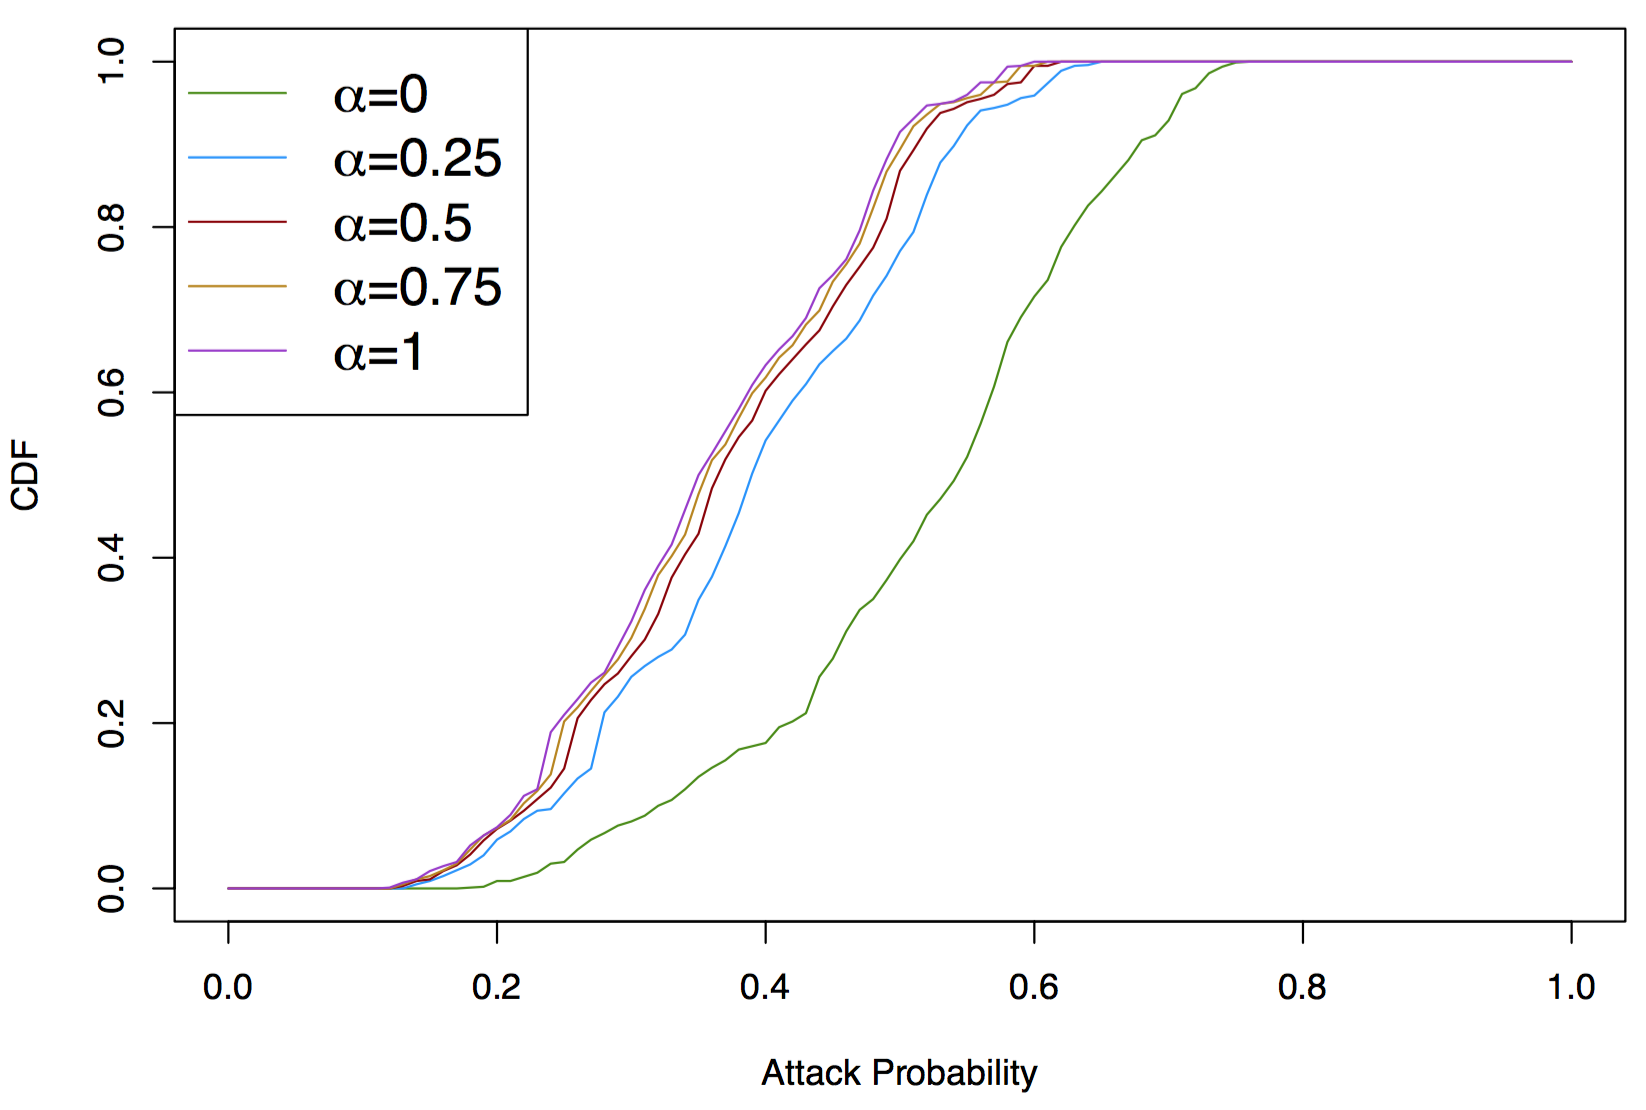
\includegraphics[width=80mm]{figure/attack}
\caption{Attack Probability with different $\alpha$ values \label{fig_attack}}
\end{figure}

We can see that $\alpha=1$ has the lowest probability of being affected by an attack, while it's pretty close to other $\alpha$ values. All of them have much lower probability compared to bandwidth-only selection. 

